\PassOptionsToPackage{unicode=true}{hyperref} % options for packages loaded elsewhere
\PassOptionsToPackage{hyphens}{url}
%
\documentclass[12pt,a4paper]{article}

\usepackage[letterpaper]{geometry}
\usepackage{times}
\geometry{top=1.0in, bottom=1.0in, left=1.0in, right=1.0in}

\usepackage{fancyhdr}
\pagestyle{fancy}
\lhead{}
\rhead{}
\lfoot{}
\rfoot{}

\renewcommand{\headrulewidth}{0pt} 
\renewcommand{\footrulewidth}{0pt} 

%\setlength\headsep{0.333in}

\usepackage{fontspec}
\usepackage{graphicx}
\usepackage{hyperref}
\usepackage{caption}
\usepackage{indentfirst}
\usepackage{setspace}
\usepackage{float}
\usepackage{enumitem}
\usepackage{listings}
\usepackage{color}
\usepackage{xcolor}
\usepackage{tabularx}
\usepackage{amsmath}
\usepackage{amssymb}
\usepackage{siunitx}

% ===========
%\input{typoraGeneratedHeaders}

% ===========

\begin{document}

\begin{titlepage}
	\begin{center}
		\vspace*{2cm}

		\doublespacing
		\rule{\linewidth}{0.3mm}

		\textsc{
			\large
			UM-SJTU Joint Institute\\
			VE281
		}

		\rule{\linewidth}{0.3mm}


		\vspace*{3.5cm}

		{
			\Large
			\textsc{Homework 1 report}\\
		}

		\vspace*{0.2cm}

		%{
		%\large
		%\textsc{Exercise 2} \\
		%\textsc{The Hall Probe: Characteristics and Applications}
		%}



	\end{center}

	\vfill
	\normalsize

	\hspace*{1cm}
	\begin{minipage}{0.4\textwidth}
		\begin{tabular}{p{1.7cm}p{4cm}ll}
			Name: & Ren Wang \hspace*{0.6cm} {\fontspec{Hei}\selectfont 王韧} & ID: & 516370910177 \\
			\multicolumn{4}{l}{Date: \today}
		\end{tabular}
	\end{minipage}

\end{titlepage}
\newpage

\onehalfspacing
\newpage

\section{Results}

In this homework, we implemented different kinds of sorting algorithm by C++ and run it with different sizes of data sets.

To test automatically, I wrote some python codes to automate the process of generating the same input data 
file for all the six algorithms.
Finally, I use MATLAB to plot the figure with respect to the logarithm of 10 and time in seconds.

The results are as followed.

\begin{figure}[H]
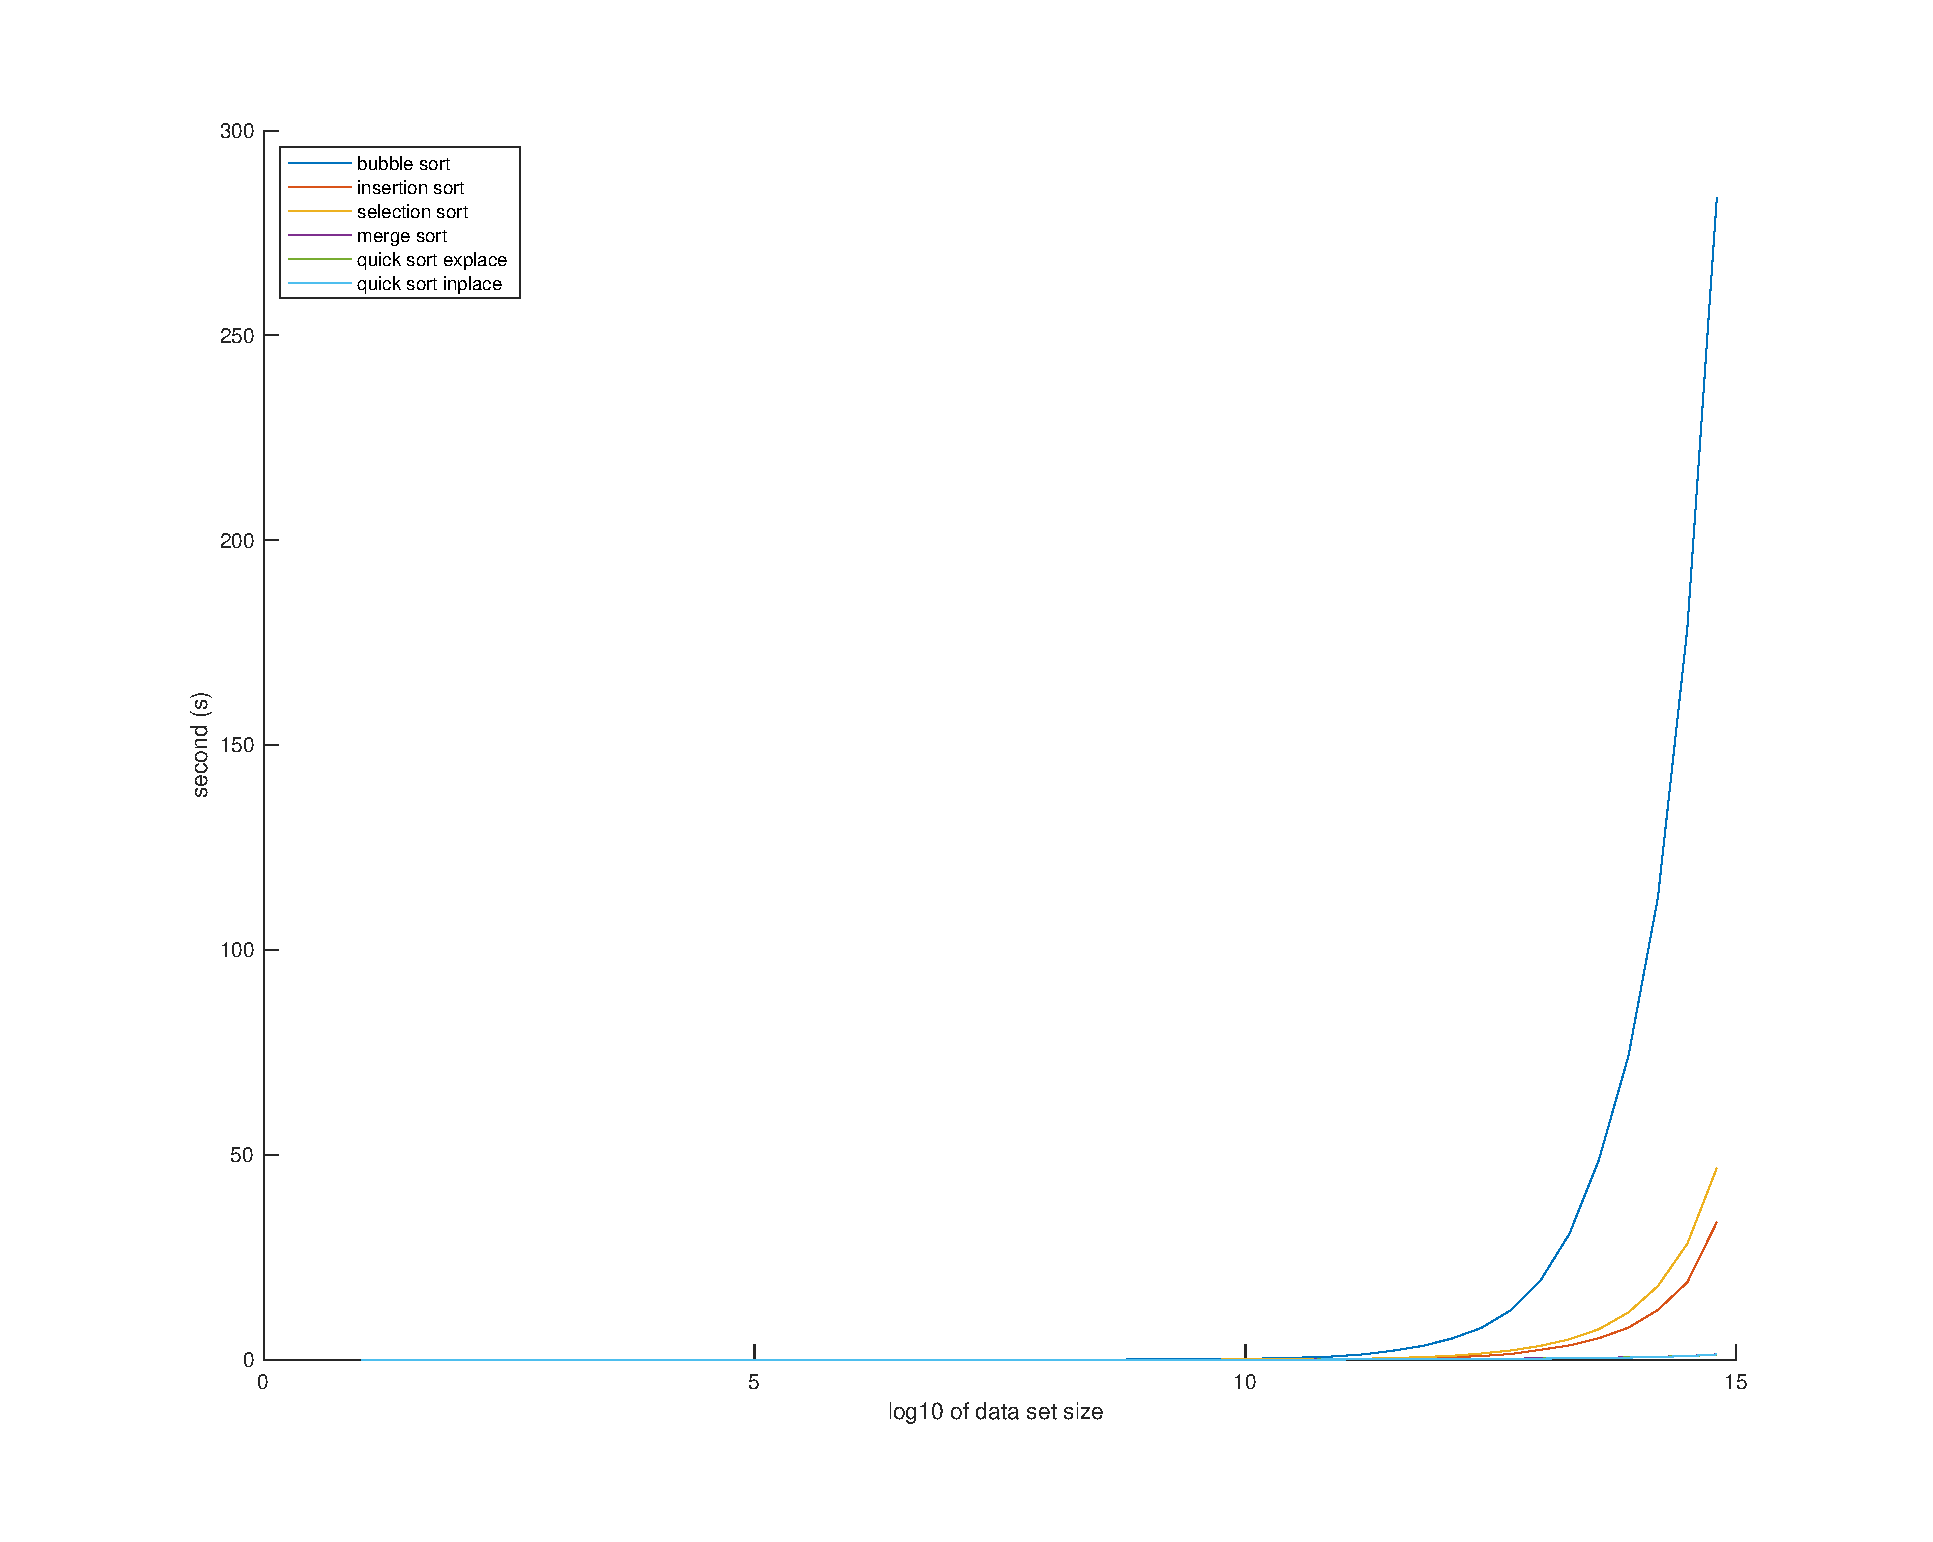
\includegraphics[width=1.1\textwidth]{lines}
\end{figure}

We can draw conclusion that bubble sort is definitely unusable when the size is big, while the two kinds of quick sort are nearly the same fast.

%\input{typoraGeneratedCode}

\end{document}

